\documentclass[tikz,border=2pt]{standalone}
\usepackage{amsmath,amssymb}
\usepackage{tikz}
\usetikzlibrary{arrows.meta}

\begin{document}
% Vehicle routing: from the depot, visit all required locations and return; with a range
% limit per trip the tour is split into several trips (two here), minimising total distance.
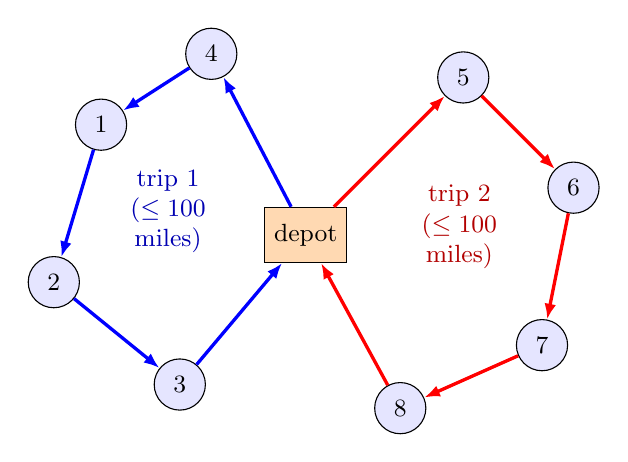
\begin{tikzpicture}[every node/.style={font=\small}, >={Latex[length=2mm]}, v/.style={draw, circle, fill=blue!10, minimum size=6.5mm, inner sep=0pt}]
	\node[draw, fill=orange!30, minimum size=7mm] (D) at (0,0) {depot};
	\node[v] (1) at (-2.6,1.4) {$1$}; \node[v] (2) at (-3.2,-0.6) {$2$}; \node[v] (3) at (-1.6,-1.9) {$3$}; \node[v] (4) at (-1.2,2.3) {$4$};
	\node[v] (5) at (2.0,2.0) {$5$}; \node[v] (6) at (3.4,0.6) {$6$}; \node[v] (7) at (3.0,-1.4) {$7$}; \node[v] (8) at (1.2,-2.2) {$8$};
	\draw[->, very thick, blue] (D) -- (4); \draw[->, very thick, blue] (4) -- (1); \draw[->, very thick, blue] (1) -- (2); \draw[->, very thick, blue] (2) -- (3); \draw[->, very thick, blue] (3) -- (D);
	\draw[->, very thick, red] (D) -- (5); \draw[->, very thick, red] (5) -- (6); \draw[->, very thick, red] (6) -- (7); \draw[->, very thick, red] (7) -- (8); \draw[->, very thick, red] (8) -- (D);
	\node[blue!70!black, align=center] at (-1.75,0.3) {trip 1\\ ($\le100$\\ miles)};
	\node[red!70!black, align=center] at (1.95,0.1) {trip 2\\ ($\le100$\\ miles)};
	\end{tikzpicture}
\end{document}
